
\documentclass[paper=a4
               ,12pt
               ,DIV=12
               ,parskip=half
               ,titlepage=on
               ,headinclude 
               ,footinclude
               %,headtopline        % Oberlinie �ber dem Kopf
               ,headsepline
               ,footsepline         % Linie unter der Kopfzeile
               ,ilines 
                %,bibtotocnumbered                           
               ]{scrartcl}
              
\usepackage[english]{babel}              % Sprachanpassungen in Klassenoptionen [english, ngerman]
\usepackage[utf8]{inputenc}   % Zeicheneingabe per Tastatur (Umlaute, etc.)
\usepackage{csquotes}           % Anf�hrungszeichen sprachenabh�ngig \enquote{}
\usepackage[T1]{fontenc}        % Schriftencoding f�r das Dokument
\usepackage{lmodern, microtype} % Bessere Trennung und Absatzkontrolle
%\usepackage[pdftex]{graphicx}   % Einbindung von Graphiken in den Formaten .pdf, .jpg, .eps
\usepackage{enumerate}
\usepackage{wrapfig}  					% Tabelle von Text umfließen lassen   
          % Grafiken von Text umfließen lassen      
\usepackage{graphicx}	
\usepackage{blindtext,              % Blindtext erzeugen
            graphicx,               % Einbinden von Graphiken (.jpg, .pdf)
            amsmath,                % Mathematikpaket
            makeidx,                % Paket f�r das Stichwortverzeichnis
            booktabs,               % Tabellenlayout-Paket
            scrpage2,
            multicol,
            pifont,
            amssymb,
            array,
            amsfonts,
            tikz,
            longtable,
            multirow,
            sidecap,
            rotating
}
% \makeatletter
%\renewcommand{\ALG@name}{Algorithmus}
%\renewcommand{\listalgorithmname}{List of \ALG@name s}
% \makeatother

\newcommand{\sign}{\text{sign}} % Signum Zeichen

 \usepackage{setspace} % Zeilenabstände definieren mit \singlespacing, \onehalfspacing          

            
\makeindex

\usepackage[
    top=3cm,
    bottom=3.5cm,
    left=2.5cm,
    right=2.5cm
    ]
    {geometry}
\linespread{1.5}

\usepackage[normalem]{ulem}

\usepackage{array}

\usepackage{hyperref}

\usepackage{tabularx}  % for 'tabularx' environment and 'X' column type
\usepackage{ragged2e}  % for '\RaggedRight' macro (allows hyphenation)
\newcolumntype{Y}{>{\RaggedRight\arraybackslash}X} 
\usepackage{booktabs}
\usepackage{color}
\usepackage{tikz}
\usetikzlibrary{shapes,arrows}

%\usepackage[pdftex,colorlinks=true,backref]{hyperref}

%\usepackage{url}

\newcommand*{\quo}[1]{{\glqq #1\grqq}}
\newcommand{\argmax}[1]{\underset{#1}{\operatorname{arg}\,\operatorname{max}}\;}
\newcommand{\argmin}[1]{\underset{#1}{\operatorname{arg}\,\operatorname{min}}\;}

\usepackage[%                       % f�r nat-Stile laden, damit \citep und \citet verf�gbar sind
           round,                  % default f�r Klammern, square, curly, angle
            %semicolon,              % Trenner f�r Mehrfachzitate: comma, semicolon
            %longnamesfirst,         % Erstes Zitat im Text mit allen Autoren
            %nonamebreak,
            %numbers             % Autoren werden nicht umgebrochen
           ]%
         {natbib}                 % Bibliographie-Paket f�r Naturwissenschaften

%\bibliographystyle{plaindin}        % Standardstile f�r das Literaturverzeichnis nach DIN: alphadin, abbrvdin, plaindin
\bibliographystyle{plainnat}         % natbib-Stile nach DIN: natdin, sonst: abbrvnat, plainnat
%\bibliographystyle{natbib}        % Stil, nahe an den Standards an der Fakult�t Statistik (nicht vorinstalliert!)




\newcommand*{\qu}[1]{{\glqq #1\grqq}}

%\usepackage{times}

\pagestyle{scrheadings}

\automark[section]{section}


\clearscrheadfoot


 \chead{}
\ihead[\headmark]{\headmark}

\ohead[\pagemark]{\pagemark}


\title{To tune or not to tune the number of trees in random forest?}    
\subject{Methodology article}
\author{Philipp Probst and Anne-Laure Boulesteix}    
\date{\today}                      
%\subject{Fallstudien I\\WS 2011/2012}         
\publishers{}               
\titlehead{Good Journal}  
\subtitle{}

\newcommand*{\Titel}[1]{\clearpage\section*{#1}\par}
\newcounter{aufgabe}
\newcommand*{\Aufgabe}{\stepcounter{aufgabe}\uline{Aufgabe~\arabic{aufgabe}:}\par} % \Alph -> \arabic
\begin{document} 
\maketitle
% Define block styles
\tikzstyle{decision} = [diamond, draw, fill=blue!20, 
    text width=4.5em, text badly centered, node distance=2.5cm, inner sep=0pt]
\tikzstyle{block} = [rectangle, draw, fill=blue!20, 
    text width=18em, text centered, rounded corners, minimum height=4em]
\tikzstyle{blockgreen} = [rectangle, draw, fill=green!20, 
    text width=18em, text centered, rounded corners, minimum height=4em]
\tikzstyle{blockred} = [rectangle, draw, fill=red!20, 
    text width=18em, text centered, rounded corners, minimum height=4em]
\tikzstyle{line} = [draw, -latex']
\tikzstyle{cloud} = [draw, rectangle,fill=red!20, node distance=6cm, text width=7em,
    minimum height=5em]

\section*{Abstract}
The random forest (RF) algorithm for supervised learning involves a number of parameters which have to be set by the users, including the number of trees to be grown as part of the forest---denoted as $T$ from now on. 
It is controversial, however, whether the number of trees should simply be set to the largest computationally manageable value or whether a smaller $T$ may in some cases be better, in which case $T$ should ideally be 
tuned carefully. This question is relevant to any user of RF and has been the topic of much informal discussion in the community, but has to our knowledge never been addressed systematically from a theoretical and empirical 
point of view. While the principle underlying bagging is that \lq\lq more trees are better'', in practice the classification error rate (in the case of classification RF) sometimes reaches a minimum before increasing 
again for increasing number of trees. 
The goal of this paper is four-fold: (i) providing theoretical results showing that the expected error rate may be a non-monotonous function of the number of trees and explaining under which circumstances this happens; 
(ii) providing theoretical results showing that such a non-monotonous pattern cannot be observed for other accuracy measures such as the Brier score or the log-loss (for classification) and the mean squared error 
(for regression); (iii) illustrating the extent of the problem through an application to a large number ($n=XXX$) of datasets from a public database; (iv) finally arguing, based on the theoretical results and empirical 
illustration, against tuning of ntree in practice or, in other words, in favor of setting ntree to the largest computationally feasible value.


\section{Introduction}

The random forest algorithm was first described in its entirety by \citet{Breiman2001}. In this paper he provides a proof for the convergence of the generalization error in the classification case for growing number of trees. 
This means that the error rate for a given test or training dataset converges to a certain value. Moreover he proofs that it exists an upper bound for the generalization error. Similarly he proofs the convergence of the mean squared generalization error for regression random forests and  
also provides an upper bound. 

These proofs did not completely solve the question if the number of trees is a tuning parameter or should be set as high as possible, although many argue intuitively for a high number of trees. 
As each tree is trained individually and without knowledge of previously trained trees, there is at least no risk of overfitting by adding more trees to the ensemble. But are there any other unknown effects?
In some applied papers \citep{Raghu2015, Barman2014} we saw that users see the 
number of trees as tuning parameters and also try different number of seeds for getting better forests \citep{Barman2014}. In the \texttt{RFmarkerDetector} R-package \citep{Palla2016} there is 
even a function to tune the number of trees. 

We initially addressed the question about the tunability by looking at the out-of-bag (OOB) error for different number of trees (also called OOB error curve) of many datasets. See also section XXX for more details on this. 
On most of the datasets we observed monotonously falling curves with growing number of trees, but in some datasets we observed strange patterns of the OOB error curves. Two of these strange error curves examples are depicted in figure 1, 
where we can see that the error rate initially steeply falls down and after a certain number of trees starts growing again until it reaches a plateau. 

\begin{figure}[!htb]
\begin{center}
  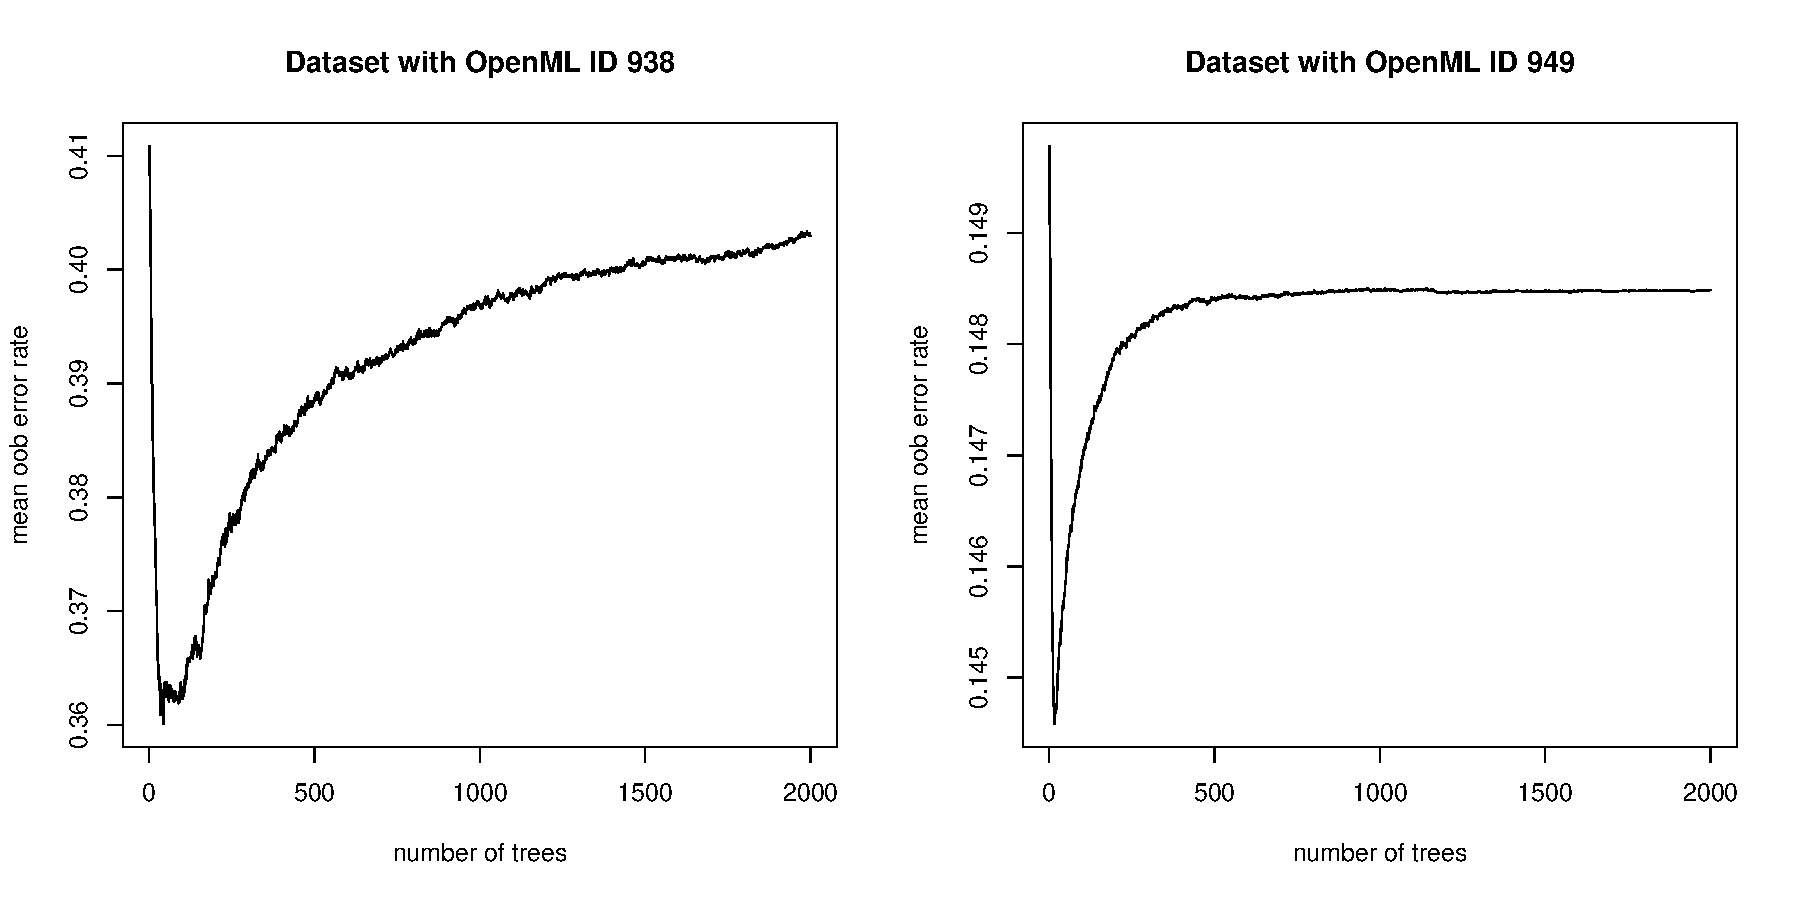
\includegraphics[width=\textwidth]{initial_example.pdf}
  \caption{Mean of OOB error curves of 1000 random forests on datasets 36 and 111}
\end{center}
\end{figure}

To address the question why this happens in some cases in section XXX we show how the generalization error looks like if the expectation of the probability of correct classification is known for each observation. 
Moreover we provide a theoretical proof in which special cases the generalization error is increasing with growing number of trees. We also proof that for other measures that use probability estimations like 
the Brier Score, the Logarithmic Loss and the AUC it always is a monotonous function and also in the regression case with the mean squared error as measure. 
In section XXX we discuss more into detail some empirical results on XXX datasets. 
Finally in the discussion section XXX we argue why nevertheless as much trees as possible should be trained to obtain a better random forest and discuss some possible automatic convergence criteria to stop automatically the
algorithm when adding a tree does not yield any substantial improvement. 

\begin{itemize}
\item Example of dataset with OOB-Error curve and OOB-Error curve with growing errorrate
\item Question: how does the distribution/expectation/variance of the OOB-curve look like?
\item Breiman proof of convergence of the generalization error
\item Paper that see ntree as tuning parameter
\begin{itemize}
\item http://journals.plos.org/plosone/article?id=10.1371/journal.pone.0133618
\item http://journals.plos.org/plosone/article?id=10.1371/journal.pone.0112034
\item Package: https://rdrr.io/cran/RFmarkerDetector/man/tuneNTREE.html
\end{itemize}
\item Literature: There is no direct paper about the development of the OOB error curve. Some papers with OOB as topic:
\begin{itemize}
\item Breiman: Random Forests
\item Breiman (2003): Out-of-Bag Estimation (this has some interesting comments)
\item Oshiro, T.M., Perez, P.S. and Baranauskas, J.A., 2012, July. How many trees in a random forest?. In MLDM (pp. 154-168): \url{http://link.springer.com.emedien.ub.uni-muenchen.de/chapter/10.1007/978-3-642-31537-4_13}
\item Mitchell: Bias of the Random Forest Out-of-Bag (OOB) Error for Certain Input Parameters
\item Ciss: Generalization Error and Out-of-bag Bounds in Random (Uniform) Forests
\item Silkes Paper...
\item  P. Latinne, O. Debeir, C. Decaestecker, Limiting the number of
trees in random forests
\item Khan: An Ensemble of Optimal Trees for Classification and Regression (OTE)
\end{itemize}
\item Stackoverflow: 
\begin{itemize}
\item \url{http://stackoverflow.com/questions/18541923/what-is-out-of-bag-error-in-random-forests}
\item What parameters to tune in random forest \url{http://stats.stackexchange.com/questions/53240/practical-questions-on-tuning-random-forests}
\item They say here that less trees could be better (stupidly): \url{http://stats.stackexchange.com/questions/36165/does-the-optimal-number-of-trees-in-a-random-forest-depend-on-the-number-of-pred/36183#36183}
\item Different seeds yield different results: \url{http://stats.stackexchange.com/questions/222279/should-random-forests-based-on-same-data-but-different-random-seeds-be-compared/222771#222771}
\item Number of trees as tuning parameter: \url{http://stats.stackexchange.com/questions/50210/caret-and-randomforest-number-of-trees}
\item Random forest overfit: \url{http://stats.stackexchange.com/questions/183973/how-not-to-overfit-a-random-forest-in-r}, \url{http://stats.stackexchange.com/questions/144305/should-you-tune-ntree-in-the-random-forest-algorithm}
\item OOB vs. CV: \url{http://stats.stackexchange.com/questions/198839/evaluate-random-forest-oob-vs-cv/199201#199201}
\item Growing OOB-curve: \url{http://stats.stackexchange.com/questions/183569/random-forest-out-of-bag-error-increases-with-number-of-trees}
\item OOB sample size: \url{http://stats.stackexchange.com/questions/173520/random-forests-out-of-bag-sample-size}
\item Relation to other parameters: \url{http://stackoverflow.com/questions/34997134/random-forest-tuning-tree-depth-and-number-of-trees}
\item Research-Gate Question: \url{https://www.researchgate.net/post/How_to_determine_the_number_of_trees_to_be_generated_in_Random_Forest_algorithm}
\end{itemize}
\end{itemize}

%\clearpage
\section{Related Work}
\citet{Oshiro2012} made a similar but not so extensive and not theoretical analysis and compared the AUC for random forests with different numbers of trees on 29 datasets. 
They concluded, that after having trained a certain number of trees (in their case 128) for the random forest the AUC performance gain of adding trees is minimal. 

\section{Background: random forest and measures of accuracy}
\subsection{Random forest}

(Mainly from Raphaels Paper)

The random forest (RF) is an ensemble learning technique consisting of the aggregation of a large number of decision 
trees, resulting in a reduction of variance compared to the single decision trees. In this paper we consider the original 
version of RF first described by \citep{Breiman2001}, while acknowledging that other variants exist, for example RF based
on conditional inference trees (CITE Hothorn, 2016) which address the problem of variable selection bias investigated 
by (CITE Strobl, 2008) or extremely randomized trees \citep{Geurts2006}. Also CITE new OTE algorithm!.

Each tree of the random forest is built based on a bootstrap sample drawn randomly from the original dataset using the CART 
method and the Gini impurity as the splitting criterion. During the building of each tree of the forest, at 
each split, only a given number of variables are considered. Random forest is 
considered a black-box algorithm, as gaining insight on a RF model is hard due to the huge number of trees. Some methods 
specific to the random forest exist to gain information, probably the most important being the variable importance. 
Another problem is the transportability of the random forest, as no convention exists on the implementation of the algorithm.

\subsection{The number of trees}
The number of trees

\subsection{Out-of-bag error}

The out-of-bag error is calculated by using the OOB estimations for the training observations. OOB estimations are calculated by predicting the class or probability for each training observation by 
using only the trees, for which the observation was not used. These estimations are compared to the real values by calculating some performance measure like e.g. the mean missclassification error 
which is the empirical counterpart of the generalization error. 

%To obtain more stable results and better estimations for the generalization error we repeated this procedure 100 times and averaged them. 

\subsection{Performance evaluation}
We now consider a fixed training dataset $D$ consisting on $n$ observations, which is used to derive prediction rules by applying the RF algorithm with a number $T$ of trees.
Ideally, the performance of these prediction rules is estimated based on an independent test dataset, denoted as $D_{test}$, consisting of $n_{test}$ test observations.

Let $e_{it}$ be an index function with 
\begin{equation}
   e_{it} =
   \begin{cases}     1 & \text{if observation } i \text{ from\ }D_{test}\ \text{ is classified correctly by tree t,}  \\
     0 & \text{otherwise,}
   \end{cases}
\end{equation}

If no test data are available, 


\section{Theoretical results}
In this section we compute the expected accuracy of a random forest consisting of $T$ trees as estimated based on the $n_{test}$ observations, while considering the training dataset as fixed. 
We also are only looking at the binary classification case, although the generalisation to multiclass classification is straightforward.

\subsection{Error rate}

Let $p_i$ be the be the expected error rate for observation $i$, $i = 1,...,n$ and number of trees $T \rightarrow \infty$. 

so that $p_i := E(e_{it})$. $p_i$ can be estimated through the fraction of trees that missclassify $i$ for a big number of trees $T$. The error rate for the whole dataset for a random forest with $T$ trees and the typical threshold 0.5 
can then be calculated as 

\begin{equation}
 Err(T) = \frac{1}{n} \sum_{i=1}^{n} I ((\frac{1}{T} \sum_{t=1}^T e_{it} ) > 0.5) = \frac{1}{n} \sum_{i=1}^{n} I ((\sum_{t=1}^T e_{it} ) > 0.5 \cdot T), 
\end{equation}

with $e_{it} \sim B(n, p_i)$ distributed like a binomial distributed variable with probability $p_i$. 

So for the expectation of this error rate, called generalisation error in \citet{Breiman2001}, we have

\begin{equation}
 E(Err(T)) = \frac{1}{n} \sum_{i=1}^{n} E( I ((\sum_{t=1}^T e_{it} ) > 0.5 \cdot T)) = \frac{1}{n} \sum_{i=1}^{n} P(X_i > 0.5 \cdot T)
\end{equation}

with $X_i=\sum_{t=1}^Te_{it}\sim\mathcal{B}(T,p_i)$. 

This is an increasing function in $T$ for $p_i > 0.5$ and a decreasing function in $T$ for $p_i < 0.5$. 
In fact if $\frac{1}{T} \sum_{t=1}^T e_{it}  = 0.5 \cdot T$ the standard implementation in R (\texttt{randomForest}) assigns the observation randomly to a class, 
but we disregard this case here as it will not change the results substantially. We could just add the term to the equations in case of an odd number of trees. 

Error curves for one observation with the mentioned adjustment in the case of odd number of trees and for different $p_i$ can be seen in figure 2. Very high and very low numbers of $p_i$ converge very quickly, while $p_i$ near 0.5 take 
longer time to converge. 

\begin{figure}[!htb]
\begin{center}
  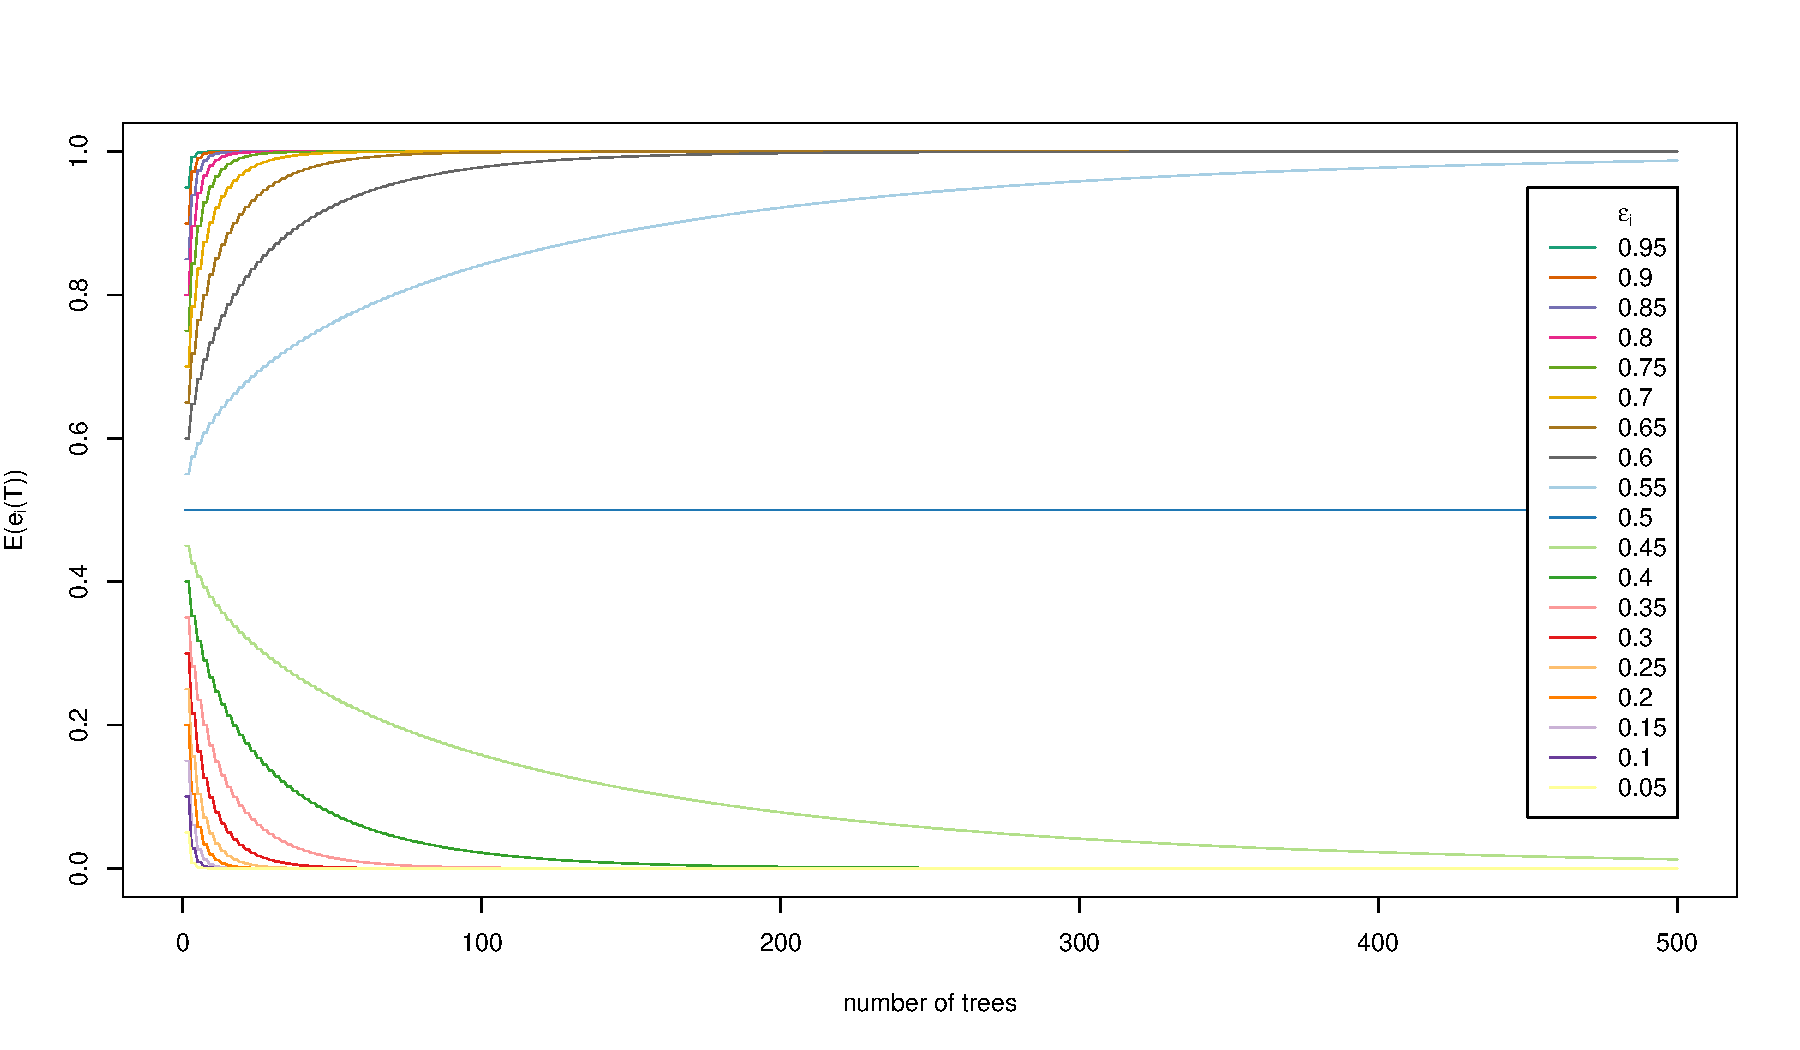
\includegraphics[width=\textwidth]{error_curves.pdf}
  \caption{Generalization error for one observation and different $p_i$ values}
\end{center}
\end{figure}

The error curve is the addition of the error curves of the single observations. Of course a good classificator should classify most observations correctly with $p_i < 0.5$. 
But if there are many observations with  $p_i$ near $0$ and some observations with $p_i > 0.5$ but near 0.5 the error curve 
will be falling down first quickly because of the observation with $p_i$ near $0$ and then grow again slowly as the number of trees increase because of the observations $p_i > 0.5$ and near 0.5. In the empirical section 
we show that this is the case for the two cases mentioned in the introduction. 

\subsubsection{Convergence speed of the error curve}
We see, that the convergence of the error curve is only dependent on the distribution of the $p_i$ of the observations. So the convergence speed of the error curve is not directly dependent 
on the number of observations $n$ or the number of features, but these characteristics could possibly influence the distribution and hence the convergence speed.  

In the empirical section we will try to look at typical distributions of the $p_i$. We will also argue why it is better to look at Brier Score and AUC curves 
and propose a reasonable convergence stop criteria that takes that into account.



%In general it is common sense, that the number of trees should be set as high as possible in random forests. In this paragraph I will show,
%that not in every data specific case a growing number of trees is leading to a better expectation mean missclassification error. This has to do with the averaging 
%procedure of the random forest, where at the end the class is chosen for which most of the trees have voted. 

\subsection{Philipps old proof (possibly remove this)}

I will show an example where the expectation of the missclassification error will be worse with higher number of trees.
For simplification this example has binary outcome and only one observation is predicted, generalisation is straightforward. 

\subsubsection{Proof}
The aim is to predict the class of one observation $x$ with binary outcome, $x \in \{0,1\}$.
Let $\hat{x}_i$ be the class prediction of tree $i$, $i = 1,...,n$, which only can take values 1 or 0. 
Let the true value of the observation $x$ be 1 and the probability of the prediction of this class by $\hat{x}_i$ be $p$ with $p<0.5$. %given a particular training sample \textbf{s}. 
The predictions of the trees are independent of each other, as each tree is trained independently of the others. 

Then we have following expectation of a true prediction (and hence of the accuracy) in the case of one tree: 
\begin{equation}
\text{E}(I(\hat{x}_1 = x)) = p. 
\end{equation}
Let $\hat{x}_n^{mod} = \mod \{\hat{x}_1, \hat{x}_2, , ... , x_n\}$ be the prediction of a forest with $n$ trees. 
In the case of two trees we can have two different predictions and so the modus is not clearly defined so we just jump to the case with three trees $\hat{x}_3^{mod}$. 

 $\hat{x}_3^{mod}$ follows a binomial distribution with probability 
 \begin{equation}
 \text{E}(I(\hat{x}_3^{mod} = x)) = p^3 +  p^2 \cdot (1-p) \cdot \binom{3}{2}.
\end{equation}

In general we have 
\begin{equation}
 \text{E}(I(\hat{x}_n^{mod} = x)) = \sum_{k= \lceil{n/2\rceil}}^n \binom{n}{k} p^k (1-p)^{n - k}
\end{equation}
which in the case of $p<0.5$ is a strictly monotonous falling function in $n$ (for uneven $n$) and converges to zero for $n \to \infty$ (to be proven, not too complicated). 

\subsubsection{Further remarks}
So the expectation for the mean missclassification error (=1-accuracy) is strictly growing in $n$ and converging to 1, so less trees are better in this specific example. 
Of course a good classificator should classify observations correctly with $p>0.5$, so this only happens in special cases were enough observations are classified wrongly. 

\clearpage 

\subsection{Brier Score}

With $w_{it} := 1-e_{it}$ ($\hat{p}_i$ is probability estimation for $y_i$):
\begin{align}
 E(\text{Brier}(T)) & = \frac{1}{n} \sum_{i=1}^{n} E((y_i - \hat{p}_i ) ^2) \nonumber \\
                    & = \frac{1}{n} \sum_{i=1}^{n} E((1 - \frac{1}{T} \sum_{t=1}^{T} e_{it} ) ^2) \nonumber \\
                    & = \frac{1}{n} \sum_{i=1}^{n} E((\frac{1}{T} \sum_{t=1}^{T} \underbrace{(1 - e_{it})}_{w_{it}} ) ^2) \nonumber \\
                    & = \frac{1}{n} \sum_{i=1}^{n} E((\frac{1}{T} \sum_{t=1}^{T} w_{it} )^2)  \nonumber
\end{align} 
Hinweis für $y_i = 0$ einfügen. 
 How is $\frac{1}{T} \sum_{t=1}^{T} w_{it} $ distributed? 
 \begin{align}
 &\sum_{t=1}^{T} w_{it} \sim \mathcal{B}(T, 1 - p_i) \nonumber \\
 &\Rightarrow Var(\sum_{t=1}^{T} w_{it}) = T \cdot p_i \cdot (1-p_i)  \nonumber \\
 &\Rightarrow Var( \frac{1}{T} \sum_{t=1}^{T} w_{it}) = \frac{1}{T} \cdot p_i \cdot (1-p_i) \\
 & \text{and }  E( \frac{1}{T} \sum_{t=1}^{T} w_{it}) = 1-p_i
\end{align}

With $Var(X) = E(X^2) - E(X)^2$ it follows:
\begin{equation} 
E((\frac{1}{T} \sum_{t=1}^{T} w_{it} )^2) = Var( \frac{1}{T} \sum_{t=1}^{T} w_{it}) - E( \frac{1}{T} \sum_{t=1}^{T} w_{it})^2 \stackrel{(7), (8)}{=} \frac{1}{T} \cdot p_i \cdot (1-p_i) + (1-p_i)^2 \nonumber
\end{equation}
This is a strictly monotonous falling function in $T$, so the expectation of the Brier score (sum of all expectations of all observations) is a strictly monotonous falling function in $T$. 

\subsection{Logarithmic Loss}

\begin{align}
E(\text{Logloss}(T)) & = -\frac{1}{n} \sum_{i=1}^{n} E(y_i \ln(\hat{p}_i) + (1 - y_i) \ln(1-\hat{p}_i)) \nonumber \\
                     & = -\frac{1}{n} \sum_{i=1}^{n} ( E(y_i \ln(\hat{p}_i)) + E ((1 - y_i) \ln(1-\hat{p}_i))) \nonumber
\end{align}

For $y_i = 1$ and one observation we obtain: 
\begin{equation}
E(\text{Logloss}(T)) =  -E(y_i \ln(\hat{p}_i)) =  -E(\ln(\hat{p}_i)) = -E(\ln(\hat{p}_i)) = -E(\ln(\frac{1}{T} \sum_{t=1}^{T} e_{it} )) \nonumber
\end{equation}
Analogously for $y_i = 0$:
\begin{equation}
E(\text{Logloss}(T)) = -E(\ln(\frac{1}{T} \sum_{t=1}^{T} e_{it} )) \nonumber
\end{equation}

With the Taylor Expansion ($\mu_X := E(X)$) (cite, e.g. Statistical theory with engineering applications, Hald, 1952),
\begin{align}
E\left[f(X)\right]  {} = & E\left[f(\mu_X + \left(X - \mu_X\right))\right] \nonumber \\
\approx & E \left[f(\mu_X) + f'(\mu_X)\left(X-\mu_X\right) + \frac{1}{2}f''(\mu_X) \left(X - \mu_X\right)^2 \right] \nonumber \\
 = & f(E(X)) + \frac{f''(E(X))}{2} \cdot Var(X) \nonumber
\end{align}

and supposing that $\frac{1}{T} \sum_{t=1}^{T} e_{it}$ is never 0, which can 
be achieved by adding a very small value to it in case it would be 0, like e.g. done in \texttt{mlr}, we obtain:

\begin{equation}
E(\text{Logloss}(T)) \approx -\ln(p_i) + \frac{\frac{1}{T} p_i (1-p_i)}{2 p_i} = -\ln(p_i) + \frac{1-p_i}{2T}, \nonumber
\end{equation}
which is a decreasing function in T.

Passt das so???

(Jensen's inequality does not help here).

\subsection{AUC}

The expectation of the AUC...

\subsection{MSE}

With prediction $\hat{y}_{i} = \frac{1}{T} \sum_{t=1}^{T} \hat{y}_{it}$ for observation $i$ after training $T$ trees: 
\begin{align}
 E(\text{MSE}(T)) & = E(\frac{1}{n} \sum_{i=1}^{n} (y_i - \hat{y}_i) ^ 2) \nonumber \\
                  & = \frac{1}{n} \sum_{i=1}^{n} E((y_i - \hat{y}_i) ^ 2) \nonumber
\end{align}

 \begin{align}
& E(y_i - \hat{y}_i) = b_i \\
& Var(y_i - \hat{y}_i)  = Var(\hat{y}_i) = \frac{1}{T} Var(\hat{y}_{it}) \\
& \stackrel{(9), (10)}{\Rightarrow} E((y_i - \hat{y}_i) ^ 2) = \frac{1}{T} Var(\hat{y}_{it}) + b_i^2
\end{align}
$(11)$ is a strictly monotonous falling in T, so the expectation of the MSE is a strictly monotonous falling function in $T$. 


\section{Empirical results}

\begin{itemize}
 \item Simple example with dataset comparing true with empirical results for test data (what happens when even number of trees?)
 \item Approximation of the mean/expected curve in case of oob data with correction of T (exp(-1))
 \item Analyse general structure in datasets (In x \% of the datasets we see this structure)
 \item Comparison 50 trees with 1000 trees: Accuracy can decrease with growing number of trees.
Brier Score, Logarithmic Loss, AUC and MMCE are always getting better. -> see code, maybe add this to the theoretical section
\end{itemize}

\subsection{Structure of the OOB error curve on 193 datasets}

To analyse the frequency of the problem of the growing OOB error curve we analysed the OOB error curve on 193 small datasets. We downloaded the datasets with predefined 
tasks from the OpenML platform and only chosed datasets with less than 1000 observations and less than 1000 features. We also applied some other cleaning procedures, like e.g. 
deleting datasets that appeared twice or more to get a decent subset of datasets. 
For each dataset we run 1000 random forest with the R package \texttt{randomForest} \citep{Liaw2002} and extracted the OOB error curve, which is automatically calculated by the package. 
We calculated the mean of the curves for the 1000 runs. The graphs can be seen in the annex/figshare in XXX. 
We observed, that for most datasets the curve is quickly falling down until it reaches a certain convergence value. On some few datasets (10.36 \%) it is growing again after falling down ($\equiv$ At 2000 trees the error rate is 0.005 bigger than 
the minimum value over all number of trees) and on some very few datasets (3.6 \%) it is growing from the beginning ($\equiv$ the minimum lies within the first 20 trees). This mainly happens for smaller datasets, 
from the 7 datasets where this occurs 6 belong to the smaller datasets (regarding number of observations multiplicated by number of features). 

We also looked at some histograms of the OOB probabilities of the correct classification for a random forest with a huge number of trees (100000) for the datasets with curves that are partially growing. 
These probabilities can be seen as a good approximation of the probability of correct classification of some specific observation by one tree.  
A typical example of the histogram in the case of non-monotonous error rate can be seen in figure XXX. The histograms belong to the datasets 36 and 111 for which the OOB error curve was already depicted in the introduction in figure 1. 
For dataset 111 we included the histogram of values that where between 0.1 and 0.9 to see the relevant probabilities. In both cases we see, that we have a bigger amount of observations, that have a probability that is a bit smaller than 0.5
of being correctly classified than a bit bigger than 0.5 and hence concording with our theoretical results it follows that with growing number of trees these only nearly correctly classified observations will be wrongly classified and hence 
increase the error rate when enough trees are added to the ensemble. 

\begin{figure}[!htb]
\begin{center}
  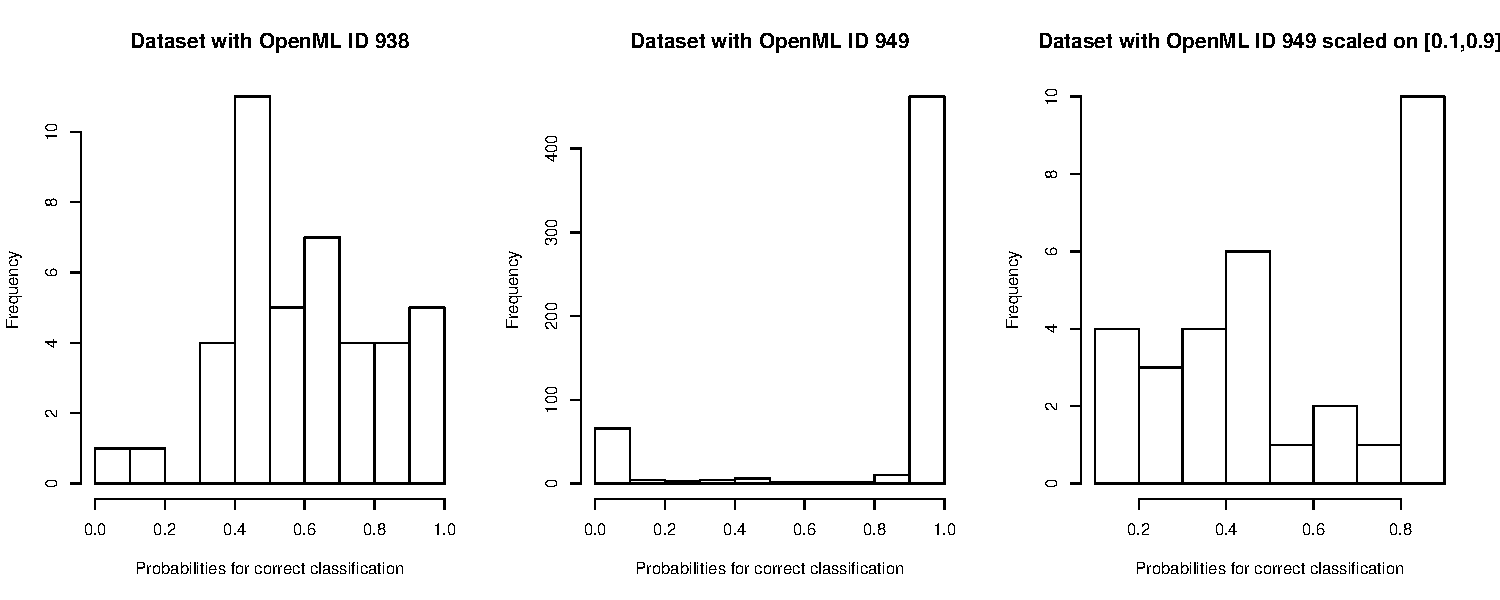
\includegraphics[width=\textwidth]{histogram.pdf}
  \caption{Histogram of the probability estimation of a random forest with 100000 trees on datasets 36 and 111}
\end{center}
\end{figure}


\section{Stopping criteria, AUC curves and Brier Score curves}


\section{Recommendation and discussion}

\begin{itemize}
 \item Generalization on any other bagging method (also with random samples of variables)
 \item Connection to the generalization error as described in Breiman
 \item Tune AUC for getting better MMCE (there was a paper about that)
 \item Why bigger ntree is always better (Reasoning...);
 \item influence (theoretical) of sampsize and tree depth (see stackoverflow post: \url{http://stackoverflow.com/questions/34997134/random-forest-tuning-tree-depth-and-number-of-trees})
 \item Other measures
 \item Multiclass and regression?
 \item Automatic break criteria, convergence measure; (Question: Are more trees needed for bigger p/n to reach convergence? (Stackoverflow question: \url{http://stats.stackexchange.com/questions/243645/maximum-tree-needed-for-random-forest-modeling})
 \item Miscellaneous: oob error rate can be used for tuning, small differences between different R-packages (e.g. show different oob-plots or aggregation scheme (randomForest: predictions, party: proportion in leaves))
\end{itemize}

\section{Conclusion}

%\begin{figure}[!htb]
%\begin{center}
%\includegraphics[width=\textwidth]{baujahr2.eps}
%\caption{Relative Häufigkeit der Anzahl an gebauten Geräten sowie der Anzahl an Geräten, für die in 2014 mindestens ein Logbuch bzw. ein Help Ticket vorliegt}
%\end{center}
%\end{figure}
\bibliography{Ntree_RandomForest}

\end{document}

%\bibliography{Ntree_RandomForest}